\documentclass[]{article}

\usepackage{polski,graphicx,comment,listings,url,colortbl,tikz}
\usepackage[utf8]{inputenc}
\usepackage{algorithm}
\usepackage{algpseudocode}
\usepackage{amsmath}
\usepackage{amssymb}
\usepackage{siunitx}
\usepackage{booktabs}
\usepackage{csvsimple}
\usepackage{pgfplots}
\usetikzlibrary{patterns}
\usepackage{placeins}

\title{Raport 4 z ECE}
\author{Paweł Ksieniewicz}


\begin{document}
\newenvironment{ride}[2]
{
	\caption{Zbiór \emph{#2}}
    \label{tab:results}
	\centering
	\begin{tabular}{lS>{\color{red}}S}
		\\\toprule{promień} & {accuracy} & {\textsc{bac}} \\\midrule
	    \csvreader[head to column names]{#1}{}%
	    {\radius & \accuracy & \bac\\}%
	\end{tabular}
	
	\begin{tikzpicture}
	\begin{axis}[
	    grid=both,
	    grid style={line width=.1pt, draw=gray!10},
	    major grid style={line width=.2pt,draw=gray!50},
	    width=6cm,
	    height=8cm,
	    xmin=0.01, xmax=0.29,
	    ymin=.0, ymax=1,
	    ytick = {.5, .6, .7, .8, .9, 1},
	    yticklabels = { ~, 60\%, ~, 80\%, ~, 100\%},
	    xtick = {0, .05, .1, 0.15, 0.2, 0.25},
		xticklabels = {~, 5,10,15,20,25},
		xlabel = Promień,
		minor tick num=2,
		xlabel style={font=\tiny,fill=white},
		ticklabel style={font=\tiny,fill=white}		]
		\addplot[color=black] table [x=radius, y=accuracy, col sep=comma] {#1};
		\addplot[color=red] table [x=radius, y=bac, col sep=comma] {#1};
	\end{axis}
	\end{tikzpicture}
}{}

\newenvironment{rideg}[2]
{
	\caption{Zbiór \emph{#2}}
    \label{tab:results}
	\centering
	\begin{tabular}{lS>{\color{red}}S}
		\\\toprule{ziarno} & {accuracy} & {\textsc{bac}} \\\midrule
	    \csvreader[head to column names]{#1}{}%
	    {\grain & \accuracy & \bac\\}%
	\end{tabular}
	
	\begin{tikzpicture}
	\begin{axis}[
	    grid=both,
	    grid style={line width=.1pt, draw=gray!10},
	    major grid style={line width=.2pt,draw=gray!50},
	    width=6cm,
	    height=8cm,
	    xmin=1, xmax=19,
	    ymin=.0, ymax=1,
	    ytick = {.5, .6, .7, .8, .9, 1},
	    yticklabels = { ~, 60\%, ~, 80\%, ~, 100\%},
	    xtick = {1, 4, 7, 10, 13, 16, 19},
		xticklabels = {~, 4,7,10,13,16,~},
		xlabel = Promień,
		minor tick num=2,
		xlabel style={font=\tiny,fill=white},
		ticklabel style={font=\tiny,fill=white}		]
		\addplot[color=black] table [x=grain, y=accuracy, col sep=comma] {#1};
		\addplot[color=red] table [x=grain, y=bac, col sep=comma] {#1};
	\end{axis}
	\end{tikzpicture}
}{}

\maketitle
\newpage

\section{ECE --- \emph{Exposer Classifier Ensemble}}

Ostatnimi czasy nurt \emph{representation learning} staje się coraz bardziej witalnym tematem badań dla środowiska uczenia maszynowego. Leżąca u jego podstaw idea twierdzi, że kluczem do skutecznej klasyfikacji trudnych zbiorów danych, jest odpowiednia ekstrakcja cech. Transformacja przestrzeni danych dostępnych w zbiorze do innej przestrzeni, w której samo zadanie się trywializuje. 

Poniższy raport prezentuje metodę transformacji przestrzeni cech, inspirowaną intuicją fotograficzną, sugerującą, że możemy wykorzystać parę cech zbioru do stworzenia \emph{wirtualnej kliszy}, którą zamiast na światło, eksponujemy na wiązkę próbek. Stąd sama jej główna struktura nazywana jest \emph{ekspozerem}.

Tak stworzone struktury, można wykorzystywać zarówno jako klasyfikatory bazowe, jak i -- kiedy decydujemy się na zbiór podzbiorów cech -- komitety klasyfikatorów. Takie podejście jest, jak w większości metod obrazowych, łatwe do zrównoleglenia, jak i niezależne od wielkości próbki, odporne na zwiększenie liczby cech zbioru uczącego, jak i pozwala na regularyzację w przestrzeni cech, przeprowadzaną niezależnie od przestrzeni oryginalnego zbioru.

Proponowana metoda została przetestowana eksperymentalnie na wyborze dziesięciu zbiorów benchmarkowych.

\subsection{\emph{Ekspozer}}
\label{exposer}

\emph{Histogram} definiujemy jako \emph{graficzną reprezentację rozkładu danych numerycznych}. Jest estymacją rozkładu prawdopodobieństwa zmiennej ciągłej, po raz pierwszy wprowadzoną przez Karla Pearsona \cite{1895RSPTA.186..343P}. 

Konstrukcja histogramu polega na podziale zakresu wartości na serię interwałów, nazywanych kubełkami i sukcesywnym zliczaniu ile wartości wpadnie do każdego z nich. Kubełki \emph{muszą być rozłączne} i z reguły są tej samej wielkości.

\emph{Scatter plot} jest rodzajem wykresu prezentującego dystrybucję dwóch cech zadanego zbioru danych. Rozkład prezentowany jest jako chmura punktów reprezentujących obiekty zbioru, z których pozycja każdego jest determinowana wartościami cech wybranych do wykresu\cite{jessica2005seeing}. Przykładowy \emph{scatter plot} dla zbioru benchmarkowego \emph{iris} można zobaczyć na Rysunku \ref{fig:scatterplots}.

Opisywana w niniejszym raporcie struktura \emph{ekspozera} czerpie zarówno z \emph{histogramu} jak i ze \emph{scatter plota}. Jak w \emph{histogramie}, zakres wartości jest dzielony na serię interwałów, ale, jak w przypadku \emph{scatter plotów}, analizowana jest nie jedna cecha, a ich para. Charakterystyczna dla histogramów reguła rozłączności jest tutaj złamana i pojedyncze obiekty mogą wpadać do więcej niż jednego kubełka. Przykładowe \emph{ekspozery}, wygenerowane dla tych samych danych, co scatter ploty w poprzedniej ilustracji, można zobaczyć na Rysunku \ref{fig:exp1}.

\begin{figure}[hbt]
	\centering
	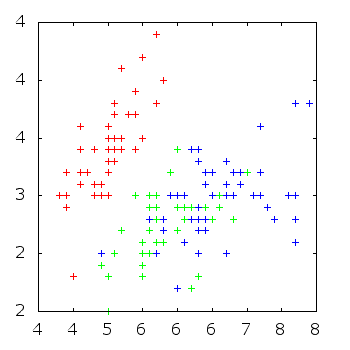
\includegraphics[width=0.32\textwidth, trim = 10 0 20 0]{figures/scatterplot_1_2}
	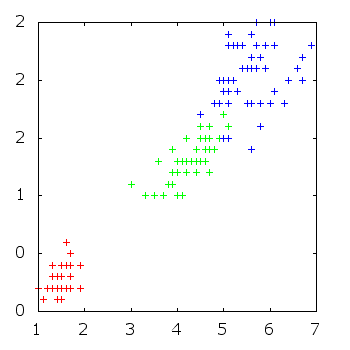
\includegraphics[width=0.32\textwidth, trim = 10 0 20 0]{figures/scatterplot_3_4}
	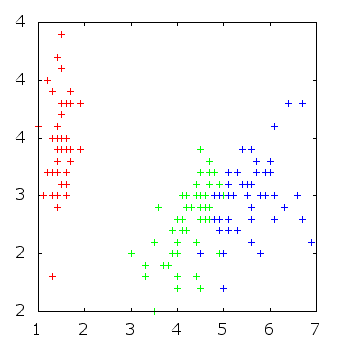
\includegraphics[width=0.32\textwidth, trim = 10 0 20 0]{figures/scatterplot_2_3}
  	\caption{Example scatter plots for \emph{iris} dataset (1:2, 3:4, 2:3)}
  	\label{fig:scatterplots}
\end{figure}

\begin{figure}[hbt]
	\centering
	
\includegraphics[width=0.305\textwidth]{figures/exponer_iris_1_2}
	
\includegraphics[width=0.305\textwidth]{figures/exponer_iris_4_3}
	
\includegraphics[width=0.305\textwidth]{figures/exponer_iris_3_2}
  	\caption{Example exposers for \emph{iris} dataset (1:2, 3:4, 2:3)}
  	\label{fig:exp1}
\end{figure}

Konstrukcja ekspozera inspirowana jest procesem naświetlania fotografii analogowej. Stąd, parametrami, które decydują o ich kształcie są:

\begin{itemize}
	\item ziarno (\verb|grain|) --- będące odpowiednikiem liczby interwałów histogramu oraz
	\item współczynnik rozproszenia światła, nazywany dalej promieniem (\verb|radius|) --- wyrażany procentowo promień oddziaływania obiektów. 
\end{itemize}

W miejsce ekspozycji kliszy fotograficznej na źródło światła, tutaj eksponujemy wielowymiarową macierz liczb na wiązkę obiektów znajdujących się w zbiorze naświetlającym. Procedura \emph{robi zdjęcie} określonemu podzbiorowi cech próbek w taki sposób, że intensywność \emph{światła} w każdym punkcie eksponowanej macierzy jest agregacją gęstości przynależności próbek do jej okolicy.

Główną różnicą wobec klasycznej fotografii, jest tutaj redefinicja samego pojęcia koloru. Dla ekspozerów, nie składa się on z klasycznych trzech kanałów modelu \textsc{rgb}\cite{svaetichin_spectral_1956}, ale tworzymy osobny wymiar spektralny dla każdej klasy występującej w zbiorze. W taki sposób otrzymujemy w strukturze dodatkowy wymiar przestrzenny, o zakresie równym sile puli klas. Proces ekspozycji macierzy każdą tak otrzymaną warstwę \emph{obrazu} uczula jedynie na obiekty reprezentujące zgodną z nią klasę. Możemy więc założyć, że efekt takiej procedury da nam reprezentację zbliżoną do obrazowania wielowidmowego \cite{1703909}. 

Algorytm \ref{alg:expose} prezentuje pseudokod procedury naświetlania macierzy ekspozera.

\begin{algorithm}[ht]
\caption{Algorytm naświetlania macierzy ekspozera}
\label{alg:expose}
\begin{algorithmic}[1]
\Procedure{expose}{objects,radius,grain,features}
	\State 
	\For{$class$ \textbf{in} $classes$}
		\State $objects' \gets objects$ \emph{labeled as} $class$
		\For{$x \gets 1$ \textbf{to} $grain$}
			\For{$y \gets 1$ \textbf{to} $grain$}
				\State $base \gets (x,y) / grain$
				\State $brightness \gets 0$	
				\For{$object$ \textbf{in} $objects'$}
					\State $base' \gets object(features)$
					\State $distance \gets \sqrt{\sum{(base' -  base)^2}}$
					\If{$distance < radius$}
						\State $brightness \gets brightness (radius - distance)$
					\EndIf
				\EndFor
				\State $\mathcal{E}[x,y,class] \gets brightness$
			\EndFor
		\EndFor
	\EndFor
\EndProcedure
\end{algorithmic}
\end{algorithm}

Aby stworzyć formalny opis algorytmu, załóżmy, że dysponujemy zbiorem $\mathcal{X}$, na który składa się $n$ próbek, po $d$ cech każda oraz $M$-elementowym zbiorem etykiet $\mathcal{M}$.

\begin{equation}
	\begin{array}[b]{llll}
		\mathcal{X} & \subseteq & \mathbb{R}^d\\
		\mathcal{M}&=&\{1, 2, \ldots, M\}\\
		x_k & = & [x_k^{(1)}, x_k^{(2)}\ldots, x_k^{(d)}],\quad x_k \in \mathcal{X}\\
		\mathcal{DS} & = & \Big\{(x_1,i_1),(x_2,i_2),\ldots,(x_n,i_n)\Big\}
	\end{array}
\end{equation}

Mamy również zbiór kombinacji $C$ z $d$ po $k$ wartościami, którego każdy element $\gamma$ ma $k$ różnych od siebie wartości.

\begin{equation}
	\begin{array}[b]{llll}
		C^k & = & \{\gamma_1^k, \ldots, \gamma_{|C^k|}^k \}\\
		\gamma_z^k & = & [x^{(t_1)}, \ldots, x^{(t_k)}], & t_1, \ldots, t_k \in \{1, \ldots, d\},\quad t_1\neq t_2 \neq \ldots \neq t_k\\
		|C^k| & = & {\;d\;\choose \;k\;}
	\end{array}
\end{equation}

A w szczególności, używając, jak np. w wypadku płaskich fotografii, kombinacji dwuelementowych,

\begin{equation}
	\begin{array}[b]{llll}
		C & = & \{\gamma_1, \ldots, \gamma_{|C|} \}\\
		\gamma_z & = & [x^{(u)}, x^{(v)}], & u, v \in \{1, \ldots, d\},\quad u\neq v\\
		|C| & = & {\;d\;\choose \;2\;}
	\end{array}
\end{equation}

Reprezentacja ekspozera $E$ jest wielowidmowym obrazem o wymiarach przestrzennych $G\times G$ i wymiarze spektralnym $M$, gdzie $G$ wyznaczane jest przez parametr ziarna, a $M$ oznacza liczbę klas w zbiorze. Ziarno przy podziale zmiennej ciągłej (lub chociaż zmiennej o niższej precyzji niż wynikałoby to z samego ziarna) zapewni realizację procesu kwantyzacji, w wielu wymiarach jednocześnie.

\begin{equation}
	\begin{array}[b]{lll}
		E^k & \in & G^k \times M\\
		E^k & = & \{ E^k_1, \ldots, E^k_M \}
	\end{array}
\end{equation}

A w szczególności,

\begin{equation}
	\begin{array}[b]{lll}
		E & \in & G \times G \times M\\
		E & = & \{ E_1, \ldots, E_M \}\\
	\end{array}
\end{equation}

Każdy punkt wyznaczony przez $g_u$ i $g_v$ skutkuje powstaniem sygnatury spektralnej $pix$.

\begin{equation}
	\begin{array}[b]{lll}
		pix(g_u,g_v) &=& [pix_1(g_u,g_v), \ldots, pix_M(g_u,g_v)]
	\end{array}
\end{equation}

Składowa pojedynczej warstwy \emph{ekspozera} (a więc monochromatyczny odpowiednik piksela w klasycznym obrazie) jest sumą wszystkich nieujemnych różnic pomiędzy zadanym promieniem oraz odległością dzielącą tzw. realny wektor centralnego punktu komórki (piksela) i wartości zadanych cech obiektów przynależących klasą do warstwy.

%\begin{equation}
%	\begin{array}[b]{lll}
%		cent(pix(g_u,g_v) &=& 
%	\end{array}
%\end{equation}

% To w zasadzie jest kwantyzacja (dyskretyzacja), na g kwantow w kazdym wymiarze przestrzennym.

\begin{equation}
	pix_i(g_u,g_v) = \sum_{k=1}^{n}\Big[d\Big(cent([g_u,g_v]),x_k\Big) < r \;\;\wedge\;\; i_k = i\Big]\;\cdot\; \Big(r - d(cent([g_u,g_v]),x_k)\Big)
\end{equation}

Powracając do metafory fotograficznej, poprzedni wzór możemy wyobrazić sobie jako projekcję przez ekspozycję, gdzie każda próbka $x_k$ jest fotonem o lokalizacji opisanej przez cechy wybrane w kombinacji $\gamma$, oddziałującym na obraz w promieniu $r$.

Taki ekspozer pozwalałby na poprawną kolorową wizualizację jedynie, gdy siła zbioru klas wynosi 3. Aby stał się uniwersalny, potrzebna jest jeszcze interpretacja \textsc{hsv} punktu \emph{ekspozera}.

\begin{equation}
	HSV(pix) = \Big[\tfrac{argmax(pix) \times 360^\circ}{M},\;max(pix) - min(pix),\;max(pix)\Big] 
\end{equation}


\subsection{\emph{Expozer} jako klasyfikator bazowy}
\label{exposerclassifier}

Wykorzystanie ekspozerów jako narzędzia klasyfikacji jest relatywnie prostym zadaniem. Załóżmy, że dysponujemy ekspozerem, naświetlonym już na zbiorze uczącym oraz próbkę $x_k$ ze zbioru testowego.

\begin{equation}
	\begin{array}[b]{l}
		x_k=\{x_k^{(1)}, x_k^{(2)}, \ldots, x_k^{(d)}\},\quad\quad x_k \in \mathcal{TS}
	\end{array}
\end{equation}

Wyliczamy lokalizację, na którą najmocniej oddziaływałaby próbka, gdyby znajdowała się ona w zbiorze uczącym.

\begin{equation}
	fin(x) = [g_u,g_v]
\end{equation}

Predykcja ($\Psi$) jest indeksem klasy o największej wartości w sygnaturze komórki macierzy korespondującej z próbką testową.

\begin{equation}
	\Psi(x_k) = \mathop{argmax}\limits_{i \in \mathcal{M}}\Bigg(pix_i\Big(fin(x_k)\Big)\Bigg)
\end{equation}

\subsection{Komitet klasyfikatorów --- \emph{Exposer} Classifier Ensemble}
\label{exposerclassifierensemble}

Aby ustanowić komitet ekspozerów, procedura predykcji potrzebuje lekkiego rozwinięcia. Załóżmy, że dysponujemy próbką $x_k$, którą chcemy sklasyfikować.

\begin{equation}
	\begin{array}[b]{cll}
		x_k &=&\{x_k^{(1)}, x_k^{(2)}, \ldots, x_k^{(d)}\},\quad\quad x_k \in \mathcal{TS}
	\end{array}
\end{equation}

Dysponujemy również zbiorem \emph{ekspozerow} ($\mathcal{E}$) zbudowanym na wszystkich $\gamma$ z $\Gamma$ możliwych do zbudowania w zbiorze uczącym.

\begin{equation}
	\begin{array}[b]{cll}
		\Gamma & \subset & C,\quad\quad |\Gamma| = N,\quad\quad N \leq {d \choose k}\\
		%\mathcal{E} & = & \{E^{(1)},\ldots,E^{(N)}\}\\
		\Pi &=& \{\Psi^{(1)},\ldots,\Psi^{(N)}\}
	\end{array}
\end{equation}

Bardziej złożony model wprowadza jednak miarę pewności decyzji wobec każdej z klas. Waga dla i-tej klasy to średnia saturacja ($S$) dla punktów odpowiadających odcieniowi klasy ($H$, $max_i(e)$) dla wartosci ($V$) większych niż zadana wielkość graniczna. 

\begin{equation}
	\theta _i = \frac{\sum_{g_u=1}^{G}\sum_{g_v=1}^{G}\Big[ argmax(pix) = i \;\wedge\; pix_i > threshold\Big]\;S(pix)}{\sum_{g_u=1}^{G}\sum_{g_v=1}^{G} \Big[ argmax(pix) = i\Big]} 
\end{equation}

\paragraph{Model klasyfikacji}

Wynikowy model klasyfikacji (Rysunek \ref{fig:model}) jest konstrukcją trójpoziomową. Na najniższym znajdują się monochromatyczne warstwy, które budują klasyfikatory składowe drugiego poziomu, określone kombinacją cech $\gamma_i$ oraz wagą $\theta_i$ używaną w metodach głosowania w obrębie komitetu. W najwyższej warstwie, klasyfikatory składowe łączone są w komitet \textsc{ece}.

\begin{figure*}[hbt]
	\center
  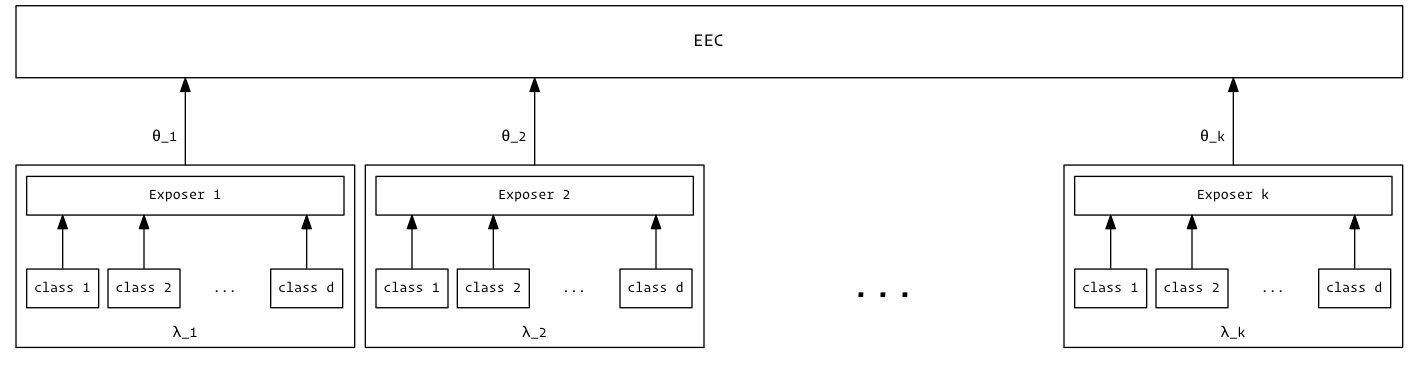
\includegraphics[width=\textwidth]{figures/ece_model}
  
  \caption{Model klasyfikacji \textsc{ece}}
	\label{fig:model}
\end{figure*}

\section{Ewaluacja eksperymentalna metody}

\subsection{Zbiory danych}

Aby zweryfikować skuteczność algorytmu, użyte zostało dziesięć baz benchmarkowych. Większość z nich pochodzi z bazy \textsc{ucimlr}\cite{asuncion2007uci} i zostały one wybrane tak, aby stworzyć możliwie różnorodną pulę problemów do rozwiązania. Selekcja została dokonana na bazie następujących wytycznych:

\begin{itemize}
	\item Zbiory powinny zawierać tak binarne (\emph{6 baz}) jak i wieloklasowe (\emph{4 bazy, po 3 i 4 klasy}) problemy do rozwiązania.
	\item Zbiory powinny być zarówno nisko, jak i wysokowymiarowe (\emph{od 4 do 35 cech}).
	\item Powinny być uwzględniane zarówno zbiory rzadkie (\emph{43 próbki dla bazy Soybean}) jak gęste (\emph{1000 próbek dla German}).
	\item Cechy analizowanych zbiorów powinny być tak ciągłe (\emph{Iris}) jak i dyskretne (\emph{Balance}).
\end{itemize}

Krótki przegląd wszystkich wybranych zbiorów zawiera się w Tabeli \ref{tab:datasets_overview}.

\begin{table*}[!ht]
	\caption{Przegląd zbiorów danych}
	\label{tab:datasets_overview}
	\centering
	\csvreader[tabular=lccc,
        table head=\toprule zbiór danych & l. cech & l. próbek & l. klas \\\midrule,
        late after line = \\,
        late after last line = \\\bottomrule]%
    {comparison.csv }{dataset=\dataset,attributes=\attributes,samples=\samples,classes=\classes}%
    {\emph{\dataset} & \attributes & \samples & \classes}%
\end{table*}

\subsection{Środowisko eksperymentalne}

Eksperyment badawczy powstał w oparciu o \emph{framework} uczenia maszynowego \textsc{ksskml}\footnote{\url{https://github.com/w4k2/KSSKML}} i został zaimplementowany jako jego rozszerzenie, udostępnione w repozytorium paczek \verb|pip| jako moduł \textsc{ece}\footnote{\url{https://github.com/w4k2/ece}}, aktualnie w wersji \oldstylenums0.\oldstylenums6.\oldstylenums3. Kod odpowiedzialny za przeprowadzenie poniższych eksperymentów, podsumowanie ich oraz tekst poniższego raportu zostały umieszczone w repozytorium w serwisie Github\footnote{\url{https://github.com/xehivs/eceReport}}.

Początkowa intuicja dotycząca algorytmu \textsc{ece} podpowiada, że istniej wysoka, ale tracąca wpływ powoli wraz ze wzrostem parametru, korelacja pomiędzy wartością \emph{ziarna} i efektywnością klasyfikacji, w związku z czym w jego testach jednostkowych była ona pierwotnie ustalona na \oldstylenums{100}. Ich rzeczywista relacja została przedstawiona na przebiegach trzech zbiorów uczących i można zaobserwować ją na Rysunku \ref{fig:grain}.

\begin{figure*}[!ht]
  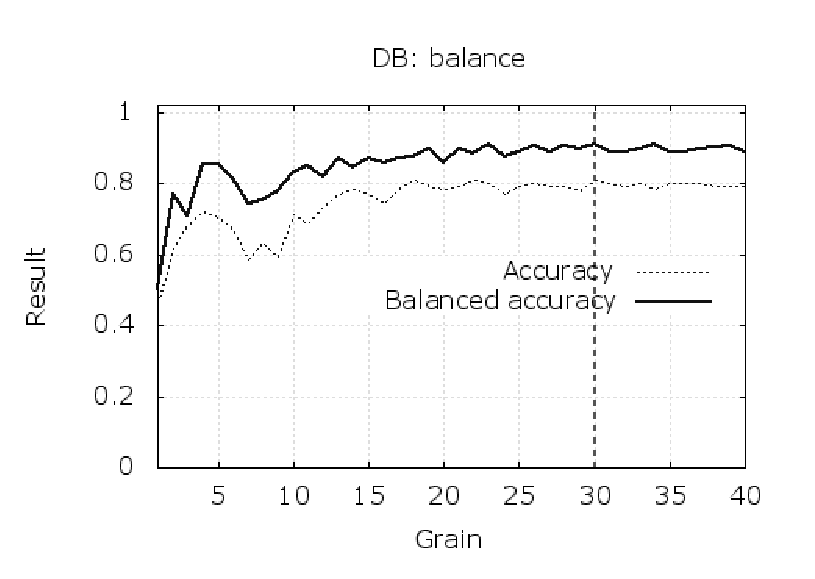
\includegraphics[width=0.32\textwidth]{figures/grain_balance}
  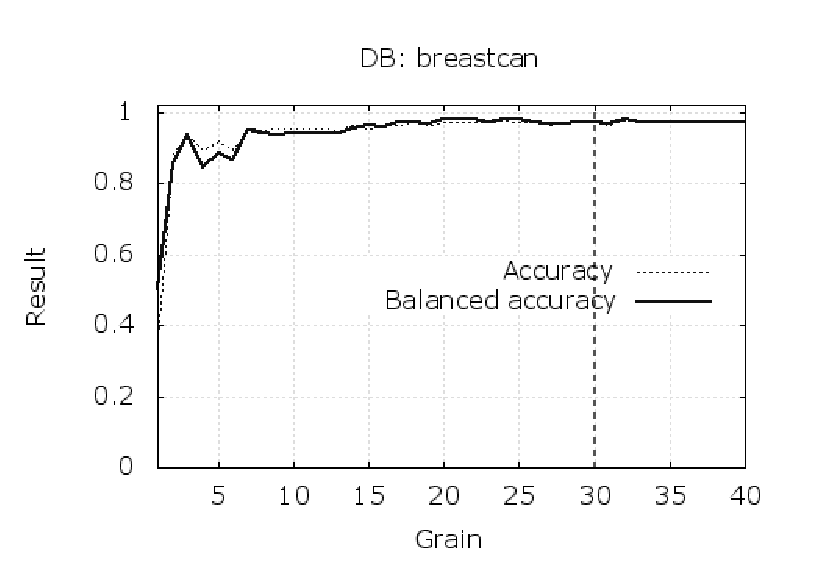
\includegraphics[width=0.32\textwidth]{figures/grain_breastcan}
  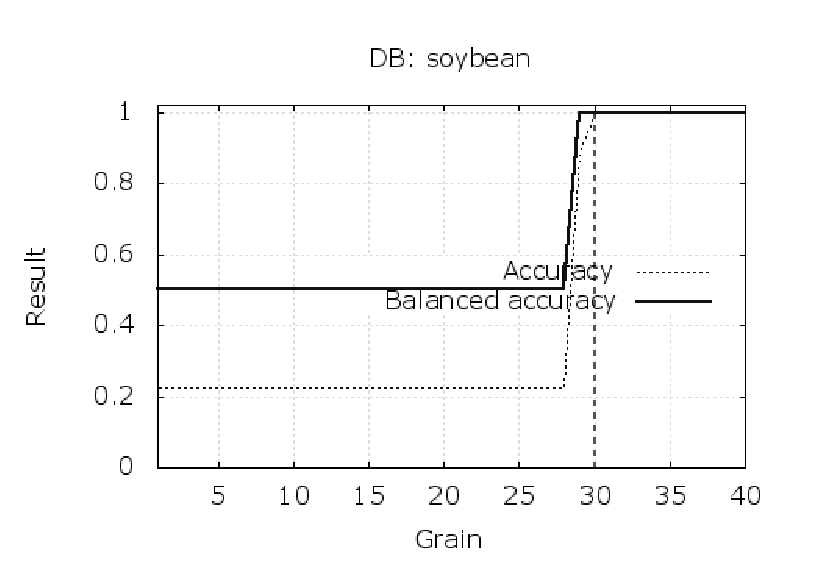
\includegraphics[width=0.32\textwidth]{figures/grain_soybean}
  
  \caption{Efektywność klasyfikacji dla stałego \emph{promienia} i zmiennego \emph{ziarna}}
	\label{fig:grain}
\end{figure*}

Zaskakująco, dla większości zbiorów (podobnie jak w przypadku \emph{Breastcan}) algorytm osiąga swoją maksymalną zdolność dyskryminacji dla \emph{ziarna} w okolicach \oldstylenums{10}. Jakkolwiek, dla części zbiorów (np. \emph{Soybean}), należyta klasyfikacja jest możliwa dopiero po osiągnięciu nieco większej wartości tego parametru (\oldstylenums{25}--\oldstylenums{30}). Wreszcie, w niektórych przypadkach (\emph{Balance}), po początkowym wczesnym wzroście efektywności następuje regresja i dopiero późniejsza stabilizacja efekywności. Wybraną wartością, która wydaje się dostatecznym kompromisem, było ziarno ustalone na \oldstylenums{15}. 

Ustalenie wartości \emph{limitu} również na \oldstylenums{15} skutkuje stworzeniem modelu o wielkości maksimum \oldstylenums{52}.\oldstylenums{5} \emph{kilobajta} na klasę (\oldstylenums{105} \emph{kilobajtów} dla problemu binarnego, \oldstylenums{210} dla dwuklasowego). Jakkolwiek, maksymalna wielkość jest osiągana jedynie, jeśli w analizowanym problemie występuje co najmniej sześć cech. W mniejszych i równych problemach, algorytm dokonuje przeglądu zupełnego wśród wszystkich możliwych kombinacji.

\subsection{Rezultaty}

\subsubsection{Badanie wpływu promienia}

Tabele 2--11 przedstawiają wyniki osiągnięte przez algorytm dla \emph{ziarna} \oldstylenums{15} i parametrów \emph{promienia} z przedziału \oldstylenums{1}--\oldstylenums{30}. Testy zostały przeprowadzone z wykorzystaniem walidacji krzyżowej \oldstylenums5v\oldstylenums2.

\begin{table*}[htb]
    \sisetup{round-mode=places}
    \sisetup{
    	round-precision = 3,
    	round-integer-to-decimal
    }
    \parbox{.45\linewidth}{
	    \begin{ride}{products/r_australian.csv}{Australian}\end{ride}
	}
	\hfill
    \parbox{.45\linewidth}{
	    \begin{ride}{products/r_balance.csv}{Balance}\end{ride}
	}
\end{table*}

\begin{table*}[!ht]
    \sisetup{round-mode=places}
    \sisetup{
    	round-precision = 3,
    	round-integer-to-decimal
    }
    \parbox{.45\linewidth}{
	    \begin{ride}{products/r_breastcan.csv}{Breastcan}\end{ride}
	}
	\hfill
    \parbox{.45\linewidth}{
	    \begin{ride}{products/r_diabetes.csv}{Diabetes}\end{ride}
	}
\end{table*}


\begin{table*}[!ht]
    \sisetup{round-mode=places}
    \sisetup{
    	round-precision = 3,
    	round-integer-to-decimal
    }
    \parbox{.45\linewidth}{
	    \begin{ride}{products/r_german.csv}{German}\end{ride}
	}
	\hfill
    \parbox{.45\linewidth}{
	    \begin{ride}{products/r_hayes.csv}{Hayes}\end{ride}
	}
\end{table*}

\begin{table*}[!ht]
    \sisetup{round-mode=places}
    \sisetup{
    	round-precision = 3,
    	round-integer-to-decimal
    }
    \parbox{.45\linewidth}{
	    \begin{ride}{products/r_heart.csv}{Heart}\end{ride}
	}
	\hfill
    \parbox{.45\linewidth}{
	    \begin{ride}{products/r_ionosphere.csv}{Ionosphere}\end{ride}
	}
\end{table*}

\begin{table*}[!ht]
    \sisetup{round-mode=places}
    \sisetup{
    	round-precision = 3,
    	round-integer-to-decimal
    }
    \parbox{.45\linewidth}{
	    \begin{ride}{products/r_iris.csv}{Iris}\end{ride}
	}
	\hfill
    \parbox{.45\linewidth}{
	    \begin{ride}{products/r_soybean.csv}{Soybean}\end{ride}
	}
\end{table*}

\FloatBarrier


\subsubsection{Badanie wpływu ziarna}

Tabele 2--23 przedstawiają wyniki osiągnięte przez algorytm dla \emph{promienia} \oldstylenums{9} i parametrów \emph{ziarna} z przedziału \oldstylenums{1}--\oldstylenums{30}. Testy zostały przeprowadzone z wykorzystaniem walidacji krzyżowej \oldstylenums5v\oldstylenums2.

\begin{table*}[htb]
    \sisetup{round-mode=places}
    \sisetup{
    	round-precision = 3,
    	round-integer-to-decimal
    }
    \parbox{.45\linewidth}{
	    \begin{rideg}{products/g_australian.csv}{Australian}\end{rideg}
	}
	\hfill
    \parbox{.45\linewidth}{
	    \begin{rideg}{products/g_balance.csv}{Balance}\end{rideg}
	}
\end{table*}

\begin{table*}[!ht]
    \sisetup{round-mode=places}
    \sisetup{
    	round-precision = 3,
    	round-integer-to-decimal
    }
    \parbox{.45\linewidth}{
	    \begin{rideg}{products/g_breastcan.csv}{Breastcan}\end{rideg}
	}
	\hfill
    \parbox{.45\linewidth}{
	    \begin{rideg}{products/g_diabetes.csv}{Diabetes}\end{rideg}
	}
\end{table*}


\begin{table*}[!ht]
    \sisetup{round-mode=places}
    \sisetup{
    	round-precision = 3,
    	round-integer-to-decimal
    }
    \parbox{.45\linewidth}{
	    \begin{rideg}{products/g_german.csv}{German}\end{rideg}
	}
	\hfill
    \parbox{.45\linewidth}{
	    \begin{rideg}{products/g_hayes.csv}{Hayes}\end{rideg}
	}
\end{table*}

\begin{table*}[!ht]
    \sisetup{round-mode=places}
    \sisetup{
    	round-precision = 3,
    	round-integer-to-decimal
    }
    \parbox{.45\linewidth}{
	    \begin{rideg}{products/g_heart.csv}{Heart}\end{rideg}
	}
	\hfill
    \parbox{.45\linewidth}{
	    \begin{rideg}{products/g_ionosphere.csv}{Ionosphere}\end{rideg}
	}
\end{table*}

\begin{table*}[!ht]
    \sisetup{round-mode=places}
    \sisetup{
    	round-precision = 3,
    	round-integer-to-decimal
    }
    \parbox{.45\linewidth}{
	    \begin{rideg}{products/g_iris.csv}{Iris}\end{rideg}
	}
	\hfill
    \parbox{.45\linewidth}{
	    \begin{rideg}{products/g_soybean.csv}{Soybean}\end{rideg}
	}
\end{table*}

\FloatBarrier

\subsection{Podsumowanie}

Na podstawie zaprezentowanych przebiegów można zaobserwować, że w wybranym zakresie promienia, jeśli ziarno ustalimy na relatywnie niedużej wartości, zależność pomiędzy nim a efektywnością klasyfikacji jest znacznie słabsza niż w wypadku tej z testów wstępnych.

Tabele \ref{tab:accuracy} oraz \ref{tab:bac} przedstawiają najlepsze osiągi dla każdej bazy testowej, względem \emph{accuracy} i \emph{balanced accuracy}, dla problemów wieloklasowych wyliczonego jako średnia z testów \emph{jeden kontra wszyscy}. 

\begin{table*}[!ht]
	\sisetup{round-mode=places}
    \sisetup{
		round-precision = 3,
		round-integer-to-decimal
	}
    \parbox{.45\linewidth}{   
		\caption{Najlepszy \emph{promień} względem accuracy}
	    \label{tab:accuracy}
		\centering
		\begin{tabular}{lSS}
			\toprule
			{zbiór danych} & {promień} & {accuracy} \\\midrule
		    \csvreader[head to column names]{products/acc.csv}{}%
		    {\emph{\filename} & \radiusr & \accuracyr\\}
		\end{tabular}
	}
	\hfill
	\parbox{.45\linewidth}{
		\caption{Najlepszy \emph{promień} względem \textsc{bac}}
	    \label{tab:bac}
		\centering
		\begin{tabular}{lS>{\color{red}}S}
			\toprule
			{zbiór danych} & {promień} & {\textsc{bac}} \\\midrule
		    \csvreader[head to column names]{products/bac.csv}{}%
		    {\emph{\filename} & \radiusr & \bacr\\}
		\end{tabular}
	}
	
	 \parbox{.45\linewidth}{   
		\caption{Najlepsze \emph{ziarno} względem accuracy}
	    \label{tab:accuracy}
		\centering
		\begin{tabular}{lSS}
			\toprule
			{zbiór danych} & {ziarno} & {accuracy} \\\midrule
		    \csvreader[head to column names]{products/acc.csv}{}%
		    {\emph{\filename} & \graing & \accuracyg\\}
		\end{tabular}
	}
	\hfill
	\parbox{.45\linewidth}{
		\caption{Najlepsze \emph{ziarno} względem \textsc{bac}}
	    \label{tab:bac}
		\centering
		\begin{tabular}{lS>{\color{red}}S}
			\toprule
			{zbiór danych} & {ziarno} & {\textsc{bac}} \\\midrule
		    \csvreader[head to column names]{products/bac.csv}{}%
		    {\emph{\filename} & \graing & \bacg\\}
		\end{tabular}
	}
	
    \parbox{\linewidth}{
    	\begin{tikzpicture}
		\begin{axis}[
			    ybar,
			    width = 1.1\linewidth,
			    bar width=0.15cm,
			    height = 6cm,
			    symbolic x coords={australian, balance, breastcan, diabetes, german, hayes, heart, ionosphere, iris, soybean},			    
			    xtick=data,
			    grid=both,
			    grid style={line width=.1pt, draw=gray!10},
			    major grid style={line width=.2pt,draw=gray!50},
			    ymin=.45, ymax=1,
			    ytick = {.5, .6, .7, .8, .9, 1},
			    yticklabels = { 50\%, 60\%, 70\%, 80\%, 90\%, 100\%},
				ticklabel style={font=\tiny,fill=white},				
			    x tick label style={rotate=30,anchor=east},	
		    ]
			\addplot[black, fill=white, postaction={pattern=north east lines}] table[x=filename, y=accuracyr, col sep=comma] {products/acc.csv};
			\addplot[red, fill=white, pattern color = red, postaction={pattern=north east lines}] table[x=filename, y=bacr, col sep=comma] {products/bac.csv};
			\addplot[black, fill=white, postaction={pattern= sixpointed stars}] table[x=filename, y=accuracyg, col sep=comma] {products/acc.csv};
			\addplot[red, fill=white, pattern color = red, postaction={pattern= sixpointed stars}] table[x=filename, y=bacr, col sep=comma] {products/bac.csv};
		\end{axis}
		\end{tikzpicture}
    }
\end{table*}

Wyniki sumaryczne potwierdzają wysoką zdolność algorytmu do poprawnej klasyfikacji, przy niedużych promieniach, oscylujących w granicach \oldstylenums{10}\%.

\FloatBarrier

\section{Wnioski}

Powyższy raport prezentuje klasyfikator sformułowany jako komitet wielospektralnych obrazów generowanych na podstawie kombinowanych podzbiorów cech zbioru danych. Każdy obraz opisuje wybraną podprzestrzeń cech, a każda jego warstwa -- odnosi się do jednej klasy problemu. Podejście tego typu przejawia odporność na klątwę wymiarowości, co pozwala na efektywne przetwarzanie danych wielowymiarowych. Algorytm bez przeciwskazań może być używany do rozwiązywania realnych problemów.

\bibliographystyle{unsrt}
\bibliography{biblography}

\end{document}
